\begin{abstract}
We study long-context balanced entropic optimal transport (OT) attention on TPU hardware through a stopped-base, fixed-depth tail-refinement surrogate. After a stopped $T$-step Sinkhorn solve, we unroll a short refinement tail and differentiate that surrogate exactly. For the production $R=2$ case, the backward pass contains four staircase plan factors. We prove an exact one-reference-tile schedule: the $R=2$ score cotangent is a single reference plan tile times an explicit modifier field built from vector cotangents and dual differences. This yields block-wise cost $O((T+R)LW)$, $O(Ld)$ input storage, and $O(L)$ additional HBM usage for fixed head dimension $d$ and band width $W$. We also formalize the current \texttt{dustbin\_block} path as the same balanced surrogate on an augmented support, so the schedule lifts to the gap-aware transport path used in our TPU runs. We provide a local surrogate-bias bound, an a posteriori bias certificate, and a projective contraction certificate for strictly positive active blocks. On synthetic masked problems, the optimized kernel matches exact autodiff of the same centered surrogate to within $10^{-5}$--$10^{-10}$. On TPU v6e-8, a four-configuration Pfam screen completes end-to-end, and a promoted balanced $R=2$ run sustains roughly $8.5$ examples per second through a three-hour budget, reaching step $1437$. Held-out Pfam test shards improve reconstruction from $3.17$ to $0.99$ and sparse CE from $5.86$ to $5.69$ relative to step $0$. These results support exact fixed-depth backward theory, a theorem-matching gap-aware bridge, and trainability evidence for the production path.
\end{abstract}

\section{Introduction}

Pairwise alignment and structural matching remain central problems for sequence modeling. Classical dynamic-programming methods such as Smith--Waterman \citep{smith1981identification} provide optimal alignments but are not differentiable, so they cannot be inserted directly into end-to-end neural architectures. Entropic optimal transport (OT) offers a natural differentiable relaxation \citep{cuturi2013sinkhorn, peyre2019computational}: it replaces a discrete assignment with a smooth transport plan computed by Sinkhorn scaling.

For long-context models, however, two bottlenecks dominate. First, dense OT attention materializes $L\times L$ scores or plans, which is prohibitive at large $L$. Second, backward-pass design is difficult. Exact autodiff through many Sinkhorn steps is expensive and memory-hungry, while implicit differentiation can require large and unstable linear solves \citep{luise2018differential, bai2019deep}. The key question is therefore not only how to make OT attention differentiable, but how to make its differentiated object explicit, exact for the surrogate actually used, and compatible with accelerator kernels.

We address this with a stopped-base, fixed-depth \emph{tail-refinement surrogate}. After a stopped $T$-step balanced Sinkhorn solve, we append a short differentiable tail of depth $R$ and differentiate that surrogate exactly. The production TPU path uses $R=2$. A direct implementation of the exact $R=2$ adjoint must evaluate four distinct staircase plan factors. The signature implementation observation of the paper is that these factors lie in a single row/column scaling orbit, so each block can be evaluated from one reference transport tile plus vector modifiers, avoiding separate plan-tile formation for the remaining three terms.

\paragraph{Gap-aware bridge.}
The central factorization is balanced and fixed-support. The first extension carried in the unified manuscript is intentionally narrow: the current \texttt{dustbin\_block} path is not treated as a new OT solver, but as the same balanced surrogate on an augmented state space. This keeps the gap-aware transport path inside the algebraic orbit of the main factorization, rather than forcing a new theorem prematurely.

\paragraph{Related context.}
Our work is closest in spirit to recent efforts to make OT-style attention practical at accelerator scale, including FlashSinkhorn \citep{flashsinkhorn2026}. The comparison separates along two axes. FlashSinkhorn is an IO-aware solver for streaming entropic OT updates; our contribution is the differentiated stopped-base backward object. In particular, a direct $R=2$ adjoint must evaluate four distinct staircase plan factors, whereas our transport-orbit calculus evaluates each block from one reference transport tile plus vector modifiers. This does not replace a direct solver-level benchmark against FlashSinkhorn or a direct four-plan-adjoint kernel benchmark, both of which remain future work, and we do not claim wall-clock dominance without such benchmarks. The present paper instead establishes the exact factorized backward object and its TPU realization on the alignment stack used in our experiments. The approach is also complementary to long-context transformer architectures that obtain efficiency through structured sparsity rather than transport constraints, such as Longformer \citep{beltagy2020longformer} and BigBird \citep{zaheer2020bigbird}.

The paper makes three main contributions:
\begin{itemize}
    \item an explicit balanced fixed-support tail-refinement surrogate together with its exact $R=2$ adjoint and one-reference-tile backward schedule;
    \item a theorem-aligned dustbin augmentation showing that the current gap-aware transport path is the same balanced surrogate on an enlarged state space;
    \item an empirical bridge from exactness validation to TPU-scale training, comprising a completed four-configuration Pfam screen, a promoted long-budget balanced run, and a held-out checkpoint evaluation on Pfam test shards.
\end{itemize}

\section{Method}

\subsection{Forward Pass: Block-Wise Balanced Sinkhorn}

Let $Q,K,V$ be query, key, and value tensors with head dimension $d$, and let $\Omega$ denote a fixed active support with band width $W$. We absorb the entropic temperature $\varepsilon$ into the score matrix
\[
S_{ij} = \frac{Q_i K_j^\top}{\sqrt{d}\,\varepsilon}.
\]
The stopped base solve and the refinement tail both use the same masked balanced half-steps
\begin{align}
    u_i^{(t+1)} &= -\log\!\Bigl[\sum_{j:(i,j)\in\Omega} \exp(S_{ij} + v_j^{(t)})\Bigr], \\
    v_j^{(t+1)} &= -\log\!\Bigl[\sum_{i:(i,j)\in\Omega} \exp(S_{ij} + u_i^{(t+1)})\Bigr].
\end{align}
The implementation computes these updates in tiles, in the same spirit as IO-aware attention kernels. For fixed band width $W$, a $T$-step base solve followed by an $R$-step tail has cost $O((T+R)LW)$ time, $O(Ld)$ input storage, and $O(L)$ additional HBM usage.

\begin{remark}[Fixed-Budget \texorpdfstring{$\varepsilon$}{epsilon}-Scaling]
The implementation optionally uses a short continuation schedule $\varepsilon_1 \ge \cdots \ge \varepsilon_S = \varepsilon$ during the stopped base solve. If the stage iteration counts satisfy $\sum_{s=1}^{S} T_s = T$, the asymptotic cost remains $O(TLW)$ time and $O(L)$ additional HBM memory for fixed head dimension.
\end{remark}

\subsection{Balanced Tail Refinement and the \texorpdfstring{$R=2$}{R=2} Staircase}

Let $(u^{(0)},v^{(0)})$ be the stopped potentials produced by the base $T$-step solve. The differentiated object is not the full $T$-step map; it is the fixed-depth surrogate
\[
\widetilde O^{[R]}(Q,K,V;u^{(0)},v^{(0)}) = \mathcal{A}(Q,K,V,u^{(R)},v^{(R)}),
\]
where the refinement iterates are recomputed from the stopped base pair. The implementation stores centered dual representatives for numerical stability, while the algebra below uses ungauged representatives; Appendix~\ref{app:proofs} proves that the centered and ungauged forward recurrences are gauge-equivalent.

Define staircase plans
\[
P_{ij}^{(a,b)} =
\begin{cases}
\exp(S_{ij}+u_i^{(a)}+v_j^{(b)}), & (i,j)\in\Omega, \\
0, & (i,j)\notin\Omega.
\end{cases}
\]
Let $\mathcal{L}$ be a scalar loss depending on $\widetilde O^{[R]}$, let $G=\partial \mathcal{L}/\partial \widetilde O^{[R]}$, and define
\[
Z_{ij}=\langle G_i, V_j\rangle,
\qquad
g_u=(P^{(R,R)}\odot Z)\mathbf{1},
\qquad
g_v=(P^{(R,R)}\odot Z)^\top\mathbf{1}.
\]

\begin{proposition}[Exact Fixed-Depth Tail Adjoint]\label{prop:tail_adjoint_main}
The cotangents of the refinement duals satisfy
\begin{align}
    \bar v^{(R)} &= g_v, \\
    \bar u^{(R)} &= g_u - P^{(R,R)}\bar v^{(R)}, \\
    \bar v^{(t-1)} &= -\bigl(P^{(t,t-1)}\bigr)^\top \bar u^{(t)}, \qquad t=R,R-1,\dots,1, \\
    \bar u^{(t-1)} &= -P^{(t-1,t-1)}\bar v^{(t-1)}, \qquad t=R,R-1,\dots,2,
\end{align}
where the final line stops at $t=2$ because the base state is stop-gradient. The score-space cotangent is
\begin{equation}
\label{eq:generic_score_vjp_unified}
\bar S
=
P^{(R,R)} \odot Z
-
\sum_{t=1}^R
\Bigl[
P^{(t,t)} \odot \bigl(\mathbf{1}\bar v^{(t)\top}\bigr)
+
P^{(t,t-1)} \odot \bigl(\bar u^{(t)}\mathbf{1}^\top\bigr)
\Bigr].
\end{equation}
\end{proposition}

For the production kernel we use $R=2$, which yields the staircase
\[
\bigl(P^{(2,2)},\,P^{(2,1)},\,P^{(1,1)},\,P^{(1,0)}\bigr).
\]

\begin{proposition}[One-Reference-Tile \texorpdfstring{$R=2$}{R=2} Backward Schedule]\label{thm:single_base_main}
For any staircase pair $(a,b)\in\{(2,2),(2,1),(1,1),(1,0)\}$,
\[
P^{(a,b)}
=
P^{(2,2)}
\odot
\exp(u^{(a)}-u^{(2)})
\odot
\exp(v^{(b)}-v^{(2)}).
\]
Define
\[
\alpha_i=\exp(u_i^{(1)}-u_i^{(2)}),
\qquad
\beta_j=\exp(v_j^{(1)}-v_j^{(2)}),
\qquad
\delta_j=\exp(v_j^{(0)}-v_j^{(2)}).
\]
Then on the active support the exact $R=2$ score-space VJP is
\[
\bar S_{ij}
=
P^{(2,2)}_{ij}
\Bigl[
Z_{ij}
-\bar v^{(2)}_j
-\beta_j\bar u^{(2)}_i
-\alpha_i\beta_j\bar v^{(1)}_j
-\alpha_i\delta_j\bar u^{(1)}_i
\Bigr].
\]
Hence, for a $B\times B$ score tile, the exact backward can be scheduled with one resident reference plan tile $P^{(2,2)}_{I,J}$, the corresponding $O(B)$ vector slices, and the $O(Bd)$ activation/cotangent slices needed to form $S_{I,J}$ and $Z_{I,J}$. The remaining staircase factors are never formed as resident plan tiles. For fixed block size, head dimension, band width, $T$, and $R=2$, the schedule uses $O(Ld)$ input storage, $O(L)$ global vector state, and $O(LW)$ tile arithmetic for the tail backward.
\end{proposition}

For $R=2$, equation~\eqref{eq:generic_score_vjp_unified} expands to
\begin{align}
\bar S
&=
P^{(2,2)} \odot Z
-
P^{(2,2)} \odot \bigl(\mathbf{1}\bar v^{(2)\top}\bigr)
-
P^{(2,1)} \odot \bigl(\bar u^{(2)}\mathbf{1}^\top\bigr) \nonumber \\
&\qquad
-
P^{(1,1)} \odot \bigl(\mathbf{1}\bar v^{(1)\top}\bigr)
-
P^{(1,0)} \odot \bigl(\bar u^{(1)}\mathbf{1}^\top\bigr).
\label{eq:r2_expanded_vjp}
\end{align}
The reconstruction identity above then replaces separate formation of the last three plan tiles with row and column rescalings of $P^{(2,2)}$.

\begin{figure}[h]
    \centering
    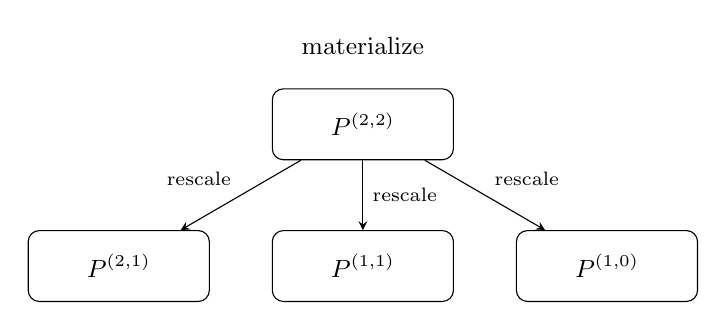
\begin{tikzpicture}[>=stealth, font=\small]
        \node[draw, rounded corners, minimum width=2.3cm, minimum height=0.9cm] (p22) at (0,0) {$P^{(2,2)}$};
        \node[draw, rounded corners, minimum width=2.3cm, minimum height=0.9cm] (p21) at (-3.1,-1.8) {$P^{(2,1)}$};
        \node[draw, rounded corners, minimum width=2.3cm, minimum height=0.9cm] (p11) at (0,-1.8) {$P^{(1,1)}$};
        \node[draw, rounded corners, minimum width=2.3cm, minimum height=0.9cm] (p10) at (3.1,-1.8) {$P^{(1,0)}$};
        \node at (0,1.0) {\small materialize};
        \draw[->] (p22) -- (p21) node[midway, above left] {\scriptsize rescale};
        \draw[->] (p22) -- (p11) node[midway, right] {\scriptsize rescale};
        \draw[->] (p22) -- (p10) node[midway, above right] {\scriptsize rescale};
    \end{tikzpicture}
    \caption{The $R=2$ staircase. Only the base plan $P^{(2,2)}$ is materialized; the remaining three plans are reconstructed from dual differences by row and column rescaling.}
    \label{fig:staircase}
\end{figure}

This schedule is the signature implementation observation in the manuscript. It converts the explicit four-factor $R=2$ backward into evaluation from one reference plan tile plus cheap row and column modifiers, which is why the method maps cleanly to TPU kernels.

\paragraph{Why \texorpdfstring{$R=2$}{R=2}.}
The multiplicative orbit identity itself is not unique to $R=2$. Relative to any chosen base staircase plan, every other staircase plan factors by the corresponding dual differences in the same way. What is special about $R=2$ is that the exact adjoint closes into the compact four-factor formula above, so the identity yields a concrete one-reference-tile schedule rather than a larger family of rescaled plans.

\subsection{Gap-Aware Dustbin Bridge}

The current gap-aware production path does not use a new OT solver. Instead, it augments the balanced problem. Let the base sequence length be $L$ and let $B=128$ denote the dustbin block size used in the implementation. Define augmented tensors
\[
\widetilde Q,\widetilde K,\widetilde V \in \mathbb{R}^{(L+B)\times d}
\]
by appending one learned dustbin token per side together with $B-1$ inactive filler tokens. The masks are augmented analogously: one appended token is active, the rest are inactive fillers. The implementation then applies the same balanced tail-refinement solver to this augmented system, with effective band width
\[
\widetilde W = \max(W,L).
\]

\begin{proposition}[Dustbin Augmentation Bridge]\label{thm:dustbin_aug}
Let $(\widetilde Q,\widetilde K,\widetilde V,\widetilde\Omega)$ denote the dustbin-augmented tensors and active support constructed above. Then the current \texttt{dustbin\_block} path is exactly the same balanced fixed-support tail-refinement surrogate as in Section~2.2, but applied on the augmented state space.
\end{proposition}

\begin{corollary}[Exact \texorpdfstring{$R=2$}{R=2} Adjoint on the Augmented State Space]\label{cor:dustbin_r2}
Apply Propositions~\ref{prop:tail_adjoint_main} and~\ref{thm:single_base_main} to the augmented system. Then the current dustbin-augmented transport path inherits the exact fixed-depth adjoint and the same one-reference-tile schedule on the augmented support.
\end{corollary}

This is the first gap-aware extension carried into the unified paper because it already matches the cloud path. It is a bridge theorem, not a departure from the central balanced factorization.

\subsection{A Local Surrogate-Bias Bound}

The fixed-depth backward is exact for the surrogate it differentiates. A separate question is how far that surrogate gradient can be from the gradient through the full stopped-base computation. Let
\[
z=(u,v),\qquad \Phi_x(z)=z^+,
\]
be the centered one-step refinement map at differentiable parameters $x$, and let $A_x(z)$ denote the transport application map. Write
\[
z_T(x)=\Phi_x^T(z_0),
\qquad
\Psi_x^R(z)=A_x\!\bigl(\Phi_x^R(z)\bigr).
\]
Then the full fixed-depth gradient is
\[
g_{\mathrm{full}}^{T,R}(x)=\nabla_x \Psi_x^R(z_T(x)),
\]
while the stop-gradient surrogate uses
\[
g_{\mathrm{surr}}^{T,R}(x)=\partial_x \Psi_x^R(z)\big|_{z=z_T(x)}.
\]

\begin{theorem}[Local Surrogate-Bias Bound]\label{thm:surrogate_bias}
Assume fixed support, $C^1$ dependence of $\Phi_x$ and $A_x$ on $(x,z)$, and constants $\rho\in[0,1)$, $L_\Phi>0$, and $L_A>0$ such that
\[
\|D_z\Phi_x(z)\|\le\rho,
\qquad
\|D_x\Phi_x(z)\|\le L_\Phi,
\qquad
\|D_z A_x(z)\|\le L_A
\]
on a forward-invariant neighborhood. Then
\[
g_{\mathrm{full}}^{T,R}(x)-g_{\mathrm{surr}}^{T,R}(x)
=
D_z\Psi_x^R(z_T(x))\,D_x z_T(x),
\]
and
\[
\bigl\|g_{\mathrm{full}}^{T,R}(x)-g_{\mathrm{surr}}^{T,R}(x)\bigr\|
\le
\frac{L_A L_\Phi}{1-\rho}\,\rho^R.
\]
\end{theorem}

The point of this bound is modest but useful: once the support is fixed and the refinement map is locally contractive, the stop-gradient bias decays geometrically in the tail depth $R$. We also record the finite-instance version used by the validation harness.

\begin{proposition}[Projective Sinkhorn Contraction Certificate]\label{prop:projective_contraction}
Consider a strictly positive active block of the balanced or dustbin-augmented support, and let
\[
K_{ij}=\exp(S_{ij})
\]
be the positive kernel on that block, using the scaled score convention from Section~2.1. For positive column scalings $c,c'$, define the two-half-step Sinkhorn scaling map
\[
\mathcal{T}(c)
=
b\oslash
\left[
K^\top
\left(a\oslash(Kc)\right)
\right],
\]
with positive marginals $a,b$; in our normalized update $a=b=\mathbf{1}$. Let $d_H$ denote Hilbert's projective metric on the positive cone and let $\Delta(A)$ be the projective diameter of a positive linear map $A$. Then
\[
d_H(\mathcal{T}(c),\mathcal{T}(c'))
\le
\rho_H\,d_H(c,c'),
\qquad
\rho_H
=
\tanh\!\left(\frac{\Delta(K)}{4}\right)
\tanh\!\left(\frac{\Delta(K^\top)}{4}\right)
<1.
\]
Equivalently, in log scalings, with $\Phi_{\mathrm{col}}(v)=\log \mathcal{T}(e^v)$ modulo additive gauge, the centered half-step pair is a contraction in oscillation seminorm:
\[
\operatorname{osc}\!\left(\Phi_{\mathrm{col}}(v)-\Phi_{\mathrm{col}}(v')\right)
\le
\rho_H\,\operatorname{osc}(v-v').
\]
If $\Omega_S=\max_{(i,j)}S_{ij}-\min_{(i,j)}S_{ij}$ on the active block, then a computable sufficient bound is
\[
\rho_H\le \tanh^2\!\left(\frac{\Omega_S}{2}\right)<1.
\]
Equivalently, for unscaled logits $\bar S$ with $S=\bar S/\varepsilon$, this reads
\[
\rho_H\le \tanh^2\!\left(\frac{\Omega_{\bar S}}{2\varepsilon}\right).
\]
\end{proposition}

This proposition is a support-local certificate, not a claim about masked zeros. The Birkhoff--Hopf argument \citep{birkhoff1957extensions,bushell1973hilbert} applies on strictly positive active blocks after masked entries and inactive dustbin fillers have been excluded. The dustbin bridge preserves the statement because the active dustbin token is part of the augmented positive block, while the inactive filler tokens are outside the cone on which the contraction is asserted.

\begin{proposition}[A Posteriori Bias Certificate]\label{prop:bias_certificate}
Let $F_R(x,z)$ denote the scalar tail objective obtained by applying the terminal loss to $A_x(\Phi_x^R(z))$, and define the measured base-state cotangent
\[
\eta_R(x)=\nabla_z F_R(x,z)\big|_{z=z_T(x)}.
\]
Then the full-gradient remainder omitted by the stopped-base surrogate is exactly
\[
\nabla_x F_R(x,z_T(x))
-
\partial_xF_R(x,z)\big|_{z=z_T(x)}
=
D_xz_T(x)^\top \eta_R(x).
\]
Consequently, for any compatible norm,
\[
\|\Delta g_R\|\le \|D_xz_T(x)^\top\|\,\|\eta_R(x)\|.
\]
\end{proposition}

This certificate is operational: $\eta_R$ is the base cotangent produced by the same fixed-depth tail reverse pass before it is discarded by the stop-gradient rule, and $D_xz_T(x)^\top\eta_R$ is a single VJP through the base Sinkhorn solve.

\begin{corollary}[Certified Tail-Depth Selection]\label{cor:certified_tail_depth}
Fix a tolerance $\tau>0$ and a maximum tail depth $R_{\max}$. For each $R\le R_{\max}$, let
\[
c_R(x)=D_xz_T(x)^\top\eta_R(x).
\]
Let $C(R)$ be any nondecreasing implementation cost over the candidate depths $\{0,\ldots,R_{\max}\}$. If the implementation chooses the first $R$ such that $\|c_R(x)\|\le \tau$ and returns the stopped-base gradient at that depth, then the returned gradient differs from full BPTT through the same $T$-step base solve by at most $\tau$. Moreover, this first feasible $R$ solves the discrete certified optimization problem
\[
\min_{0\le R\le R_{\max}} C(R)
\quad\text{subject to}\quad
\|c_R(x)\|\le \tau .
\]
If an upper bound $C_T(x)\ge\|D_xz_T(x)^\top\|$ is available, the same guarantee and optimality statement hold with the sufficient constraint $C_T(x)\|\eta_R(x)\|\le\tau$.
\end{corollary}

This turns tail-depth choice into a small certified resource-allocation problem rather than a purely heuristic hyperparameter. Instead of solving an adjoint linear system, one can either use a fixed depth such as $R=2$ when the certificate has already been calibrated, or periodically run the certificate VJP to verify that the stopped-base omission remains below a chosen tolerance.

\begin{proposition}[Transport-Orbit Calculus]\label{prop:orbit_certificate}
Consider any finite collection of transport plans $P^{(a,b)}$ generated from the same masked score tensor $S$ and the same active support, including the plans used by the $R=2$ staircase, the $T$ stopped base reverse pass, the $R$ differentiable tail reverse pass, and the certificate VJP $D_xz_T^\top\eta_R$. Fix any reference plan $P^\star=P^{(a_\star,b_\star)}$ in this collection and define
\[
r^{(a)}=\exp(u^{(a)}-u^{(a_\star)}),
\qquad
s^{(b)}=\exp(v^{(b)}-v^{(b_\star)}).
\]
Then every plan in the collection lies in the row/column scaling orbit of $P^\star$:
\[
P^{(a,b)}
=
\operatorname{diag}(r^{(a)})\,P^\star\,\operatorname{diag}(s^{(b)}).
\]
Equivalently, for any finite sum of plan-weighted score cotangent terms
\[
G=\sum_{\ell=1}^m P^{(a_\ell,b_\ell)}\odot H_\ell ,
\]
one has the single-reference representation
\[
G
=
P^\star\odot
\sum_{\ell=1}^m
\bigl(r^{(a_\ell)}(s^{(b_\ell)})^\top\bigr)
\odot H_\ell .
\]
Consequently, for fixed $T$, $R$, band width $W$, and head dimension $d$, the stopped gradient, the certified omitted-gradient VJP, and the certified tail-depth test can all be evaluated blockwise with $O((T+R)LW)$ arithmetic, $O(Ld)$ input storage, and $O((T+R)L)$ vector state, while materializing only one transport tile at a time. The compiler abstraction is therefore not a special four-plan trick: it is accumulation over a single transport orbit.
\end{proposition}

\section{Validation and Experiments}

\subsection{Exactness Validation of the Masked Surrogate}

We first separate surrogate correctness from systems scale. On synthetic masked problems for which exact autodiff through the same centered surrogate remains tractable, we compare the optimized $R=2$ kernel against a pure-JAX reference. Table~\ref{tab:exactness_unified} reports representative maximum absolute gradient deviations under the default validation setting ($\varepsilon=1$, band width $256$, $R=2$).

\begin{table}[h]
    \centering
    \begin{tabular}{@{}rrrr@{}}
        \toprule
        Length $L$ & $\max |\Delta Q|$ & $\max |\Delta K|$ & $\max |\Delta V|$ \\
        \midrule
        $512$ & $1.05 \times 10^{-5}$ & $1.73 \times 10^{-6}$ & $1.06 \times 10^{-9}$ \\
        $1024$ & $5.70 \times 10^{-6}$ & $8.13 \times 10^{-7}$ & $2.55 \times 10^{-10}$ \\
        $2048$ & $5.50 \times 10^{-6}$ & $9.17 \times 10^{-7}$ & $2.29 \times 10^{-10}$ \\
        \bottomrule
    \end{tabular}
    \caption{Maximum absolute gradient deviations between the optimized masked $R=2$ kernel and exact autodiff through the same centered surrogate.}
    \label{tab:exactness_unified}
\end{table}

Additional forward-consistency checks run through lengths $512$, $1024$, $2048$, $4096$, $8192$, and $16384$, with extended spot checks at $32768$, $65536$, and $131072$. We treat the larger checks as forward-consistency evidence rather than as exact-gradient checks.

To calibrate the local surrogate-bias discussion, we also compared tail-refinement gradients against full BPTT through the stopped-base solve on the same synthetic masked setup at $L=512$, $d=8$, $T=15$, $W=256$, and $\varepsilon=1$. Over seeds $0,1,2$, the worst-case gradient discrepancy $\max\{|\Delta Q|,|\Delta K|,|\Delta V|\}$ was $1.49\times 10^{-4}$ for $R=0$, $1.63\times 10^{-5}$ for $R=1$, $1.42\times 10^{-5}$ for $R=2$, and $1.42\times 10^{-5}$ for $R=4$. In this local exact-gradient calibration, the main empirical drop therefore occurs between zero tail refinement and the first one or two refinement steps, while $R=2$ and $R=4$ are already effectively tied at the scale of the masked validation harness.

Table~\ref{tab:bias_certificate} reports the a posteriori certificate from Proposition~\ref{prop:bias_certificate} on a smaller full-BPTT setting where the base-solve VJP can be checked directly ($L=128$, $d=8$, $T=15$, $W=128$, seeds $0,1,2$). The certificate reconstructs the full-gradient remainder to numerical precision and shows rapid decay of the measured base-state cotangent.

\begin{table}[h]
    \centering
    \begin{tabular}{@{}rrrr@{}}
        \toprule
        Tail depth $R$ & $\max\|\eta_R\|_2$ & $\max|\Delta g_R|$ & certificate residual \\
        \midrule
        $0$ & $5.89\times 10^{-3}$ & $6.29\times 10^{-4}$ & $2.47\times 10^{-10}$ \\
        $1$ & $5.40\times 10^{-4}$ & $5.93\times 10^{-5}$ & $3.64\times 10^{-11}$ \\
        $2$ & $5.47\times 10^{-5}$ & $5.33\times 10^{-6}$ & $2.84\times 10^{-11}$ \\
        $4$ & $9.03\times 10^{-7}$ & $9.99\times 10^{-8}$ & $2.74\times 10^{-11}$ \\
        \bottomrule
    \end{tabular}
    \caption{A posteriori surrogate-bias certificate. The residual is the maximum absolute difference between the actual full-vs-stopped gradient gap and the certified base-solve VJP $D_x z_T^\top\eta_R$.}
    \label{tab:bias_certificate}
\end{table}

Using the certified selector from Corollary~\ref{cor:certified_tail_depth} with max-absolute tolerance $10^{-5}$ selects $R=2$ on all three seeds in this calibration. Since the per-depth tail cost is monotone in $R$, this is the cheapest certified depth among the tested candidates and gives a certificate-level justification for using $R=2$ as the production depth in the TPU kernel.

We also validate the transport-orbit calculus from Proposition~\ref{prop:orbit_certificate} directly over all $2(T+R)$ base and tail half-step plans at $T=15,R=2,L=128$. Reconstructing every plan from the final reference plan gives maximum log-domain reconstruction error $1.91\times 10^{-6}$. Appendix~\ref{app:protocol} reports two additional diagnostics: a controlled direct-four-plan score-adjoint benchmark and projective contraction certificates computed from the promoted Pfam checkpoint.

\subsection{Short Pfam Screen on TPU v6e-8}

The first empirical bridge is the short Pfam screen on TPU v6e-8. All four core configurations complete end-to-end:
\[
\texttt{k2\_eps1},\quad
\texttt{k4\_eps1},\quad
\texttt{muot\_dustbin\_mono},\quad
\texttt{muot\_dustbin\_hybrid}.
\]
Each uses $50{,}000$ training pairs, $T=15$ base iterations, band width $1024$, and global batch size $64$. Table~\ref{tab:screen_unified} reports the step-50 screen snapshot.

\begin{table}[h]
    \centering
    \begin{tabular}{@{}lcccc@{}}
        \toprule
        Config & Step 50 Loss & Step 50 CE & Step 50 Mono & Throughput (ex/s) \\
        \midrule
        \texttt{k2\_eps1} & 3.5778 & 5.3223 & 0.3353 & 8.46 \\
        \texttt{k4\_eps1} & 3.5779 & 5.3223 & 0.3353 & 8.38 \\
        \texttt{muot\_dustbin\_mono} & 3.9030 & 5.3258 & 0.4155 & 8.41 \\
        \texttt{muot\_dustbin\_hybrid} & 4.6250 & 5.3244 & 0.4162 & 8.45 \\
        \bottomrule
    \end{tabular}
    \caption{Short TPU v6e-8 Pfam screen across the four core balanced and dustbin-augmented configurations.}
    \label{tab:screen_unified}
\end{table}

Two immediate conclusions follow. First, on the balanced path we observe no meaningful difference between $R=2$ and $R=4$ at this short-screen budget, while $R=2$ remains slightly faster. Second, the theorem-aligned dustbin bridge is operational at the same systems scale as the balanced path.

\subsection{Promoted Balanced Run}

We then promoted the balanced $\texttt{k2\_eps1}$ configuration to the longer-budget TPU training path. The full objective details are given in the protocol notes in the appendix; for the interpretation of the main text, the important point is that this promotion is a trainability and systems-stability test of the factorization-backed balanced $R=2$ path. The run reached step $1437$, repeatedly persisted checkpoints at steps $250$, $500$, $750$, $1000$, and $1250$, and sustained approximately $8.5$ examples per second after startup warmup. The initial throughput at step $0$ was $2.67$ examples per second, after which the run stabilized near $8.5$ examples per second for the remainder of the budget.

\begin{table}[h]
    \centering
    \begin{tabular}{@{}lccc@{}}
        \toprule
        Checkpoint & Reconstruction & Sparse CE & Monotonicity \\
        \midrule
        Step $0$ & 3.1742 & 5.8604 & 0.2474 \\
        Step $1437$ & 0.9881 & 5.6891 & 0.3154 \\
        \bottomrule
    \end{tabular}
    \caption{Held-out Pfam test-shard evaluation for the promoted balanced run.}
    \label{tab:heldout_promoted}
\end{table}

This promoted run should therefore be interpreted narrowly but positively. It is strong evidence that the factorization-backed balanced $R=2$ path is stable, efficient, and checkpointable under a realistic TPU budget. Table~\ref{tab:heldout_promoted} shows that the final promoted checkpoint also improves held-out reconstruction substantially and improves sparse CE modestly relative to step $0$, even though sparse CE is not optimized directly in this run. The monotonicity violation metric does not improve in this reconstruction-only run. The minibatch training loss is not monotone step-by-step, so late fluctuations in scalar loss should be read as ordinary stochastic optimization behavior rather than as an instability signal. The role of this experiment is still not to serve as a final downstream comparison against alternative attention mechanisms; it is to show that the production factorization-backed path runs cleanly over a long TPU budget and yields nontrivial held-out reconstruction improvement on the benchmark family used in the study.

\section{Discussion}

The unified picture is now clear. The core contribution remains the balanced fixed-support tail-refinement surrogate together with the exact $R=2$ one-reference-tile backward schedule. The dustbin bridge matters because it keeps the first gap-aware extension inside the same theorem family and already matches the current cloud path. The empirical evidence aligns with that theory stack: exactness holds on small masked problems, the four core balanced and dustbin-augmented screen configurations complete on TPU, and the promoted balanced path both trains cleanly through a long budget and improves held-out reconstruction and sparse CE relative to its initialization.

What remains outside the present theorem spine should stay outside it. In particular, a genuinely KL-unbalanced transport theorem, differentiable support geometry, and multimodal routing all remain reasonable follow-ons, but they are not required for the central claim of this manuscript.

\paragraph{Limitations and scope.}
The strongest limitations are deliberate. The main factorization is balanced and fixed-support; the dustbin bridge is an augmented balanced construction, not a full KL-unbalanced OT theorem. The local surrogate-bias result is local and contraction-based rather than global, and the projective contraction certificate applies to strictly positive active blocks rather than to masked zeros or disconnected supports. Empirically, the promoted long-budget run improves held-out reconstruction and sparse CE, but it is still best read as evidence of trainability and systems stability rather than as a final downstream comparison against alternative attention mechanisms, a direct FlashSinkhorn benchmark, a direct four-plan-adjoint kernel benchmark, or a CE-optimized alignment objective.

\paragraph{Broader context.}
This work is a methods and systems contribution for long-context differentiable alignment. Its immediate positive impact is to make factorization-backed OT attention practical on accelerator hardware. Its main practical costs are computational: the method still requires substantial accelerator time, and the empirical conclusions should be interpreted only within the stated benchmark scope rather than as deployment claims about downstream decision-making systems.

\section{Conclusion}

We presented a one-reference-tile backward schedule for long-context Sinkhorn attention and carried it through the first gap-aware extension that already matches the production code path. The balanced fixed-support $R=2$ schedule remains the centerpiece. The dustbin augmentation bridge lifts that schedule onto the current gap-aware transport path without changing the underlying surrogate. Exactness validation, a completed four-way TPU screen, and a promoted long-budget balanced run with held-out reconstruction and sparse-CE improvement together show that the result is not merely algebraic: it maps to a practical TPU training path.

\bibliographystyle{plainnat}
\bibliography{references}

\newpage
\appendix

\section{Balanced Tail-Refinement Proofs}
\label{app:proofs}

\paragraph{Notation.}
For the appendix proofs we work with ungauged representatives satisfying the raw masked logsumexp half-step equations. Let $\Omega$ denote the active support and define
\[
P^{(a,b)}_{ij} =
\begin{cases}
\exp(S_{ij}+u_i^{(a)}+v_j^{(b)}), & (i,j)\in\Omega, \\
0, & (i,j)\notin\Omega.
\end{cases}
\]

\begin{align}
    u_i^{(t+1)} &= -\log\!\Bigl[\sum_{j:(i,j)\in\Omega} \exp(S_{ij} + v_j^{(t)})\Bigr], \label{eq:u_update_app_unified}\\
    v_j^{(t+1)} &= -\log\!\Bigl[\sum_{i:(i,j)\in\Omega} \exp(S_{ij} + u_i^{(t+1)})\Bigr]. \label{eq:v_update_app_unified}
\end{align}

\paragraph{Centering map.}
Let $\mathbf{1}_q$ and $\mathbf{1}_k$ denote the all-ones vectors on valid queries and keys, and let
\[
m = \frac{\mathbf{1}_q}{\mathbf{1}_q^\top\mathbf{1}_q}.
\]
The implementation stores centered representatives via
\[
\mathcal{C}(u,v)=\bigl(u-(m^\top u)\mathbf{1}_q,\; v+(m^\top u)\mathbf{1}_k\bigr).
\]

\begin{lemma}[Centering Pullback]
If $(\bar u,\bar v)$ are cotangents on the outputs of $\mathcal{C}$, then
\[
\mathcal{C}^*(\bar u,\bar v)
=
\Bigl(
\bar u + m\bigl(\mathbf{1}_k^\top \bar v - \mathbf{1}_q^\top \bar u\bigr),
\;
\bar v
\Bigr).
\]
\end{lemma}

\begin{proof}
Write $s=m^\top u$, so $\delta s = m^\top \delta u$. Then
\[
\delta \mathcal{C}(u,v)
=
\bigl(\delta u-(\delta s)\mathbf{1}_q,\; \delta v+(\delta s)\mathbf{1}_k\bigr).
\]
Pairing this variation with $(\bar u,\bar v)$ and collecting coefficients of $\delta u$ and $\delta v$ yields the stated pullback.
\end{proof}

\begin{lemma}[Gauge Equivariance]
Let $\Gamma_c(u,v)=(u-c\mathbf{1}_q,\; v+c\mathbf{1}_k)$. Then the raw two-half-step map defined by equations~\eqref{eq:u_update_app_unified}--\eqref{eq:v_update_app_unified} is gauge equivariant.
\end{lemma}

\begin{proof}
Adding $c$ to every valid key potential shifts every logsumexp argument in the $u$-update by the same constant, so the update subtracts $c$ from every valid query potential. The $v$-update is identical with rows and columns swapped.
\end{proof}

\begin{proposition}[Centered-Ungauged Forward Equivalence]
Let $(\widehat u^{(t)},\widehat v^{(t)})$ be the ungauged iterates and $(u^{(t)},v^{(t)})$ the iterates produced by the centered implementation, both started from the same centered base pair. Then for every $t\ge 1$ there exists a scalar $c_t$ such that
\[
(u^{(t)},v^{(t)})=\Gamma_{c_t}\bigl(\widehat u^{(t)},\widehat v^{(t)}\bigr).
\]
Consequently the centered and ungauged implementations produce exactly the same staircase transport plans.
\end{proposition}

\begin{proof}
The claim holds at $t=1$ by definition of the centering step. Inductively, if the two previous representatives differ by a gauge transform, then gauge equivariance of the raw refinement step shows that the next raw outputs also differ by a gauge transform; applying $\mathcal{C}$ merely chooses another representative of the same orbit.
\end{proof}

\begin{lemma}[Half-Step Jacobians]
For every refinement step $t\ge 1$,
\begin{align}
    \frac{\partial u_i^{(t)}}{\partial v_j^{(t-1)}} &= -P_{ij}^{(t,t-1)}, \\
    \frac{\partial v_j^{(t)}}{\partial u_i^{(t)}} &= -P_{ij}^{(t,t)}.
\end{align}
\end{lemma}

\begin{proof}
Differentiate the masked logsumexp updates. For example,
\[
\frac{\partial u_i^{(t)}}{\partial v_j^{(t-1)}}
=
-
\frac{\exp(S_{ij}+v_j^{(t-1)})}{\sum_{k:(i,k)\in\Omega}\exp(S_{ik}+v_k^{(t-1)})}
=
-\exp(S_{ij}+u_i^{(t)}+v_j^{(t-1)})
=
-P_{ij}^{(t,t-1)}.
\]
The second identity is identical with rows and columns swapped.
\end{proof}

\paragraph{Proof of Proposition~\ref{prop:tail_adjoint_main}.}
\begin{proof}
The direct terminal transport application contributes $P^{(R,R)}\odot Z$ to $\bar S$ together with
\[
\bar v^{(R)}=g_v,
\qquad
\bar u^{(R)}=g_u-P^{(R,R)}\bar v^{(R)}.
\]
Now fix a reverse step $t\in\{1,\dots,R\}$. Pulling $\bar u^{(t)}$ back through the $u$-half-step uses the Jacobian $-P^{(t,t-1)}$:
\[
\bar v^{(t-1)} = -\bigl(P^{(t,t-1)}\bigr)^\top \bar u^{(t)},
\qquad
\bar S \mathrel{-}= P^{(t,t-1)}\odot\bigl(\bar u^{(t)}\mathbf{1}^\top\bigr).
\]
For $t\ge 2$, pulling $\bar v^{(t-1)}$ back through the $v$-half-step uses the Jacobian $-P^{(t-1,t-1)}$:
\[
\bar u^{(t-1)} = -P^{(t-1,t-1)}\bar v^{(t-1)},
\qquad
\bar S \mathrel{-}= P^{(t-1,t-1)}\odot\bigl(\mathbf{1}\bar v^{(t-1)\top}\bigr).
\]
The recursion stops at $\bar u^{(1)}$ because $u^{(0)}$ belongs to the stopped base solve. Summing the direct terminal term with the reverse-time half-step contributions yields equation~\eqref{eq:generic_score_vjp_unified}.
\end{proof}

\paragraph{Proof of Proposition~\ref{thm:single_base_main}.}
\begin{proof}
For any two staircase plans,
\[
\frac{P_{ij}^{(a,b)}}{P_{ij}^{(2,2)}}
=
\exp(u_i^{(a)}-u_i^{(2)}+v_j^{(b)}-v_j^{(2)}),
\]
which gives the exact reconstruction formula immediately. For the three non-reference factors in the $R=2$ staircase this gives
\[
P^{(2,1)}_{ij}=P^{(2,2)}_{ij}\beta_j,
\qquad
P^{(1,1)}_{ij}=P^{(2,2)}_{ij}\alpha_i\beta_j,
\qquad
P^{(1,0)}_{ij}=P^{(2,2)}_{ij}\alpha_i\delta_j.
\]
Substituting these three identities into the expanded VJP in equation~\eqref{eq:r2_expanded_vjp} and factoring out $P^{(2,2)}_{ij}$ gives
\[
\bar S_{ij}
=
P^{(2,2)}_{ij}
\Bigl[
Z_{ij}
-\bar v^{(2)}_j
-\beta_j\bar u^{(2)}_i
-\alpha_i\beta_j\bar v^{(1)}_j
-\alpha_i\delta_j\bar u^{(1)}_i
\Bigr].
\]
Thus every entry of the direct four-factor adjoint is reproduced exactly from the reference plan and vector modifiers.

For a tile $I\times J$, compute $P^{(2,2)}_{I,J}$ once from $S_{I,J}$, $u_I^{(2)}$, and $v_J^{(2)}$, compute $Z_{I,J}$ from the resident slices of $G_I$ and $V_J$, and form the bracketed modifier using only the slices of $\alpha_I$, $\bar u_I^{(2)}$, $\alpha_I\bar u_I^{(1)}$, $\beta_J$, $\delta_J$, $\bar v_J^{(2)}$, and $\beta_J\bar v_J^{(1)}$. Multiplying the single resident reference tile by this modifier yields the exact score-space VJP tile. The value-gradient term uses the same resident reference plan tile, since $\partial\mathcal L/\partial V$ receives $(P^{(2,2)}_{I,J})^\top G_I$. All subsequent propagation to $Q$ and $K$ is linear in the score cotangent tile, so it can be accumulated before the tile is evicted. The stated storage and arithmetic bounds follow by streaming over the $O(LW/B^2)$ active tiles with fixed $B$, $d$, $W$, and fixed tail depth.
\end{proof}

\section{Proofs for the Dustbin Bridge and Surrogate Bias}
\label{app:bias}

\paragraph{Proof of Proposition~\ref{thm:dustbin_aug}.}
\begin{proof}
After constructing the augmented tensors and masks, the implementation calls the same balanced Sinkhorn forward and backward path as in Section~2.2. Because only the first appended token in each dustbin block is active, every transport entry touching the remaining fillers is identically zero. Because the effective band width is $\widetilde W=\max(W,L)$, every active base token can reach the active dustbin token on the opposite side. Thus the implemented path is exactly the balanced fixed-support surrogate on an enlarged state space.
\end{proof}

\paragraph{Proof of Corollary~\ref{cor:dustbin_r2}.}
\begin{proof}
Apply Propositions~\ref{prop:tail_adjoint_main} and~\ref{thm:single_base_main} to the augmented tensors and support from Proposition~\ref{thm:dustbin_aug}. No new algebra is introduced after the augmentation itself.
\end{proof}

\paragraph{Proof of Theorem~\ref{thm:surrogate_bias}.}
\begin{proof}
By the chain rule,
\[
\nabla_x\Psi_x^R(z_T(x))
=
\partial_x \Psi_x^R(z)\big|_{z=z_T(x)}
+
D_z\Psi_x^R(z_T(x))\,D_x z_T(x),
\]
which gives the exact bias identity after subtracting the partial derivative term.

Next,
\[
D_z\Psi_x^R(z_T(x))
=
D_z A_x(z_{T+R}(x))
\prod_{r=0}^{R-1} D_z\Phi_x(z_{T+r}(x)),
\]
so
\[
\|D_z\Psi_x^R(z_T(x))\|
\le
L_A \rho^R.
\]
Differentiate the base recursion $z_{t+1}(x)=\Phi_x(z_t(x))$:
\[
D_x z_{t+1}(x)
=
D_x\Phi_x(z_t(x))
+
D_z\Phi_x(z_t(x))\,D_x z_t(x).
\]
Because $z_0$ is independent of $x$, repeated application of the norm bounds yields
\[
\|D_x z_T(x)\|
\le
L_\Phi \sum_{j=0}^{T-1}\rho^j
\le
\frac{L_\Phi}{1-\rho}.
\]
Combining the two estimates with the exact bias identity gives
\[
\bigl\|g_{\mathrm{full}}^{T,R}(x)-g_{\mathrm{surr}}^{T,R}(x)\bigr\|
\le
\frac{L_A L_\Phi}{1-\rho}\,\rho^R.
\qedhere
\]
\end{proof}

\paragraph{Proof of Proposition~\ref{prop:projective_contraction}.}
\begin{proof}
Hilbert's projective metric on the positive cone is
\[
d_H(x,y)=
\log
\frac{\max_i x_i/y_i}{\min_i x_i/y_i}.
\]
Positive diagonal scaling and coordinatewise inversion preserve this metric: diagonal scaling cancels in the coordinate ratios, and inversion swaps the maximum and minimum ratios. By the Birkhoff--Hopf theorem, any positive linear map $A$ with finite projective diameter $\Delta(A)$ satisfies
\[
d_H(Ax,Ay)
\le
\tanh\!\left(\frac{\Delta(A)}{4}\right)d_H(x,y).
\]
Decompose the two-half-step map as
\[
c
\mapsto
Kc
\mapsto
a\oslash(Kc)
\mapsto
K^\top(a\oslash(Kc))
\mapsto
b\oslash K^\top(a\oslash(Kc)).
\]
The two linear maps contribute Birkhoff--Hopf contraction factors
$\tanh(\Delta(K)/4)$ and $\tanh(\Delta(K^\top)/4)$, while the marginal scalings and inversions are projective isometries. Therefore
\[
d_H(\mathcal{T}(c),\mathcal{T}(c'))
\le
\tanh\!\left(\frac{\Delta(K)}{4}\right)
\tanh\!\left(\frac{\Delta(K^\top)}{4}\right)
d_H(c,c').
\]
Strict positivity on the active block gives finite projective diameters, hence $\rho_H<1$.

For log scalings,
\[
d_H(e^v,e^{v'})
=
\operatorname{osc}(v-v'),
\qquad
\operatorname{osc}(w)=\max_i w_i-\min_i w_i,
\]
and additive centering does not change oscillation. This gives the log-potential contraction.

Finally, for a positive matrix $K_{ij}=\exp(S_{ij})$,
\[
\Delta(K)
=
\log\max_{i,i',j,j'}
\frac{K_{ij}K_{i'j'}}{K_{ij'}K_{i'j}}
=
\max_{i,i',j,j'}
\left(S_{ij}+S_{i'j'}-S_{ij'}-S_{i'j}\right).
\]
If $\Omega_S=\max S-\min S$ on the active block, the last expression is at most $2\Omega_S$. The same bound holds for $K^\top$. Substituting into the Birkhoff--Hopf coefficient yields
\[
\rho_H
\le
\tanh^2\!\left(\frac{\Omega_S}{2}\right),
\]
and the unscaled-logit form follows from $S=\bar S/\varepsilon$.
\end{proof}

\paragraph{Proof of Proposition~\ref{prop:bias_certificate}.}
\begin{proof}
By definition,
\[
g_{\mathrm{full}}(x)=\nabla_x F_R(x,z_T(x)),
\qquad
g_{\mathrm{surr}}(x)=\partial_x F_R(x,z)\big|_{z=z_T(x)}.
\]
Applying the chain rule to the first expression gives
\[
\nabla_x F_R(x,z_T(x))
=
\partial_x F_R(x,z)\big|_{z=z_T(x)}
+
D_xz_T(x)^\top \nabla_zF_R(x,z)\big|_{z=z_T(x)}.
\]
Subtracting the stopped-base partial derivative gives the identity with $\eta_R=\nabla_zF_R(x,z_T(x))$. The norm bound follows immediately from submultiplicativity for the chosen compatible operator norm.
\end{proof}

\paragraph{Proof of Corollary~\ref{cor:certified_tail_depth}.}
\begin{proof}
Proposition~\ref{prop:bias_certificate} gives the exact identity $\Delta g_R=c_R(x)$. Therefore $\|c_R(x)\|\le\tau$ implies $\|\Delta g_R\|\le\tau$. If only an operator-norm bound $C_T(x)\ge\|D_xz_T(x)^\top\|$ is used, the bound in Proposition~\ref{prop:bias_certificate} gives
\[
\|\Delta g_R\|\le \|D_xz_T(x)^\top\|\,\|\eta_R(x)\|\le C_T(x)\|\eta_R(x)\|\le\tau.
\]
For the optimization claim, let $R^\star$ be the first feasible depth. Every smaller depth is infeasible by definition of $R^\star$, and every larger feasible depth has cost at least $C(R^\star)$ because $C$ is nondecreasing. Hence $R^\star$ minimizes $C(R)$ over the certified feasible set.
\end{proof}

\paragraph{Proof of Proposition~\ref{prop:orbit_certificate}.}
\begin{proof}
All plans in the collection use the same masked score tensor $S$ and the same active support. For any two dual pairs on that support,
\[
\frac{P_{ij}^{(a,b)}}{P_{ij}^{(a_\star,b_\star)}}
=
\exp(u_i^{(a)}-u_i^{(a_\star)}+v_j^{(b)}-v_j^{(b_\star)}),
\]
which gives the orbit formula entrywise. Multiplying this identity by $H_\ell$ and summing over $\ell$ gives the single-reference representation for $G$. The reverse recurrences in Propositions~\ref{prop:tail_adjoint_main} and~\ref{prop:bias_certificate} require only products of these plans with row or column cotangent vectors and score-space outer factors, all of which are instances of this representation. Each such product can therefore be evaluated by streaming one reference plan tile and applying the appropriate row and column multipliers. With fixed $T$, $R$, $W$, and $d$, each half-step contributes $O(LW)$ arithmetic and $O(L)$ vector state, while the input activations require $O(Ld)$ storage.
\end{proof}

\section{Experimental Protocol Notes}
\label{app:protocol}

The current manuscript uses three empirical layers:
\begin{enumerate}
    \item exactness checks against exact autodiff on small masked problems;
    \item a four-configuration TPU v6e-8 Pfam screen across balanced and dustbin-augmented paths;
    \item a promoted long-budget balanced run for the factorization-backed $R=2$ path.
\end{enumerate}

All TPU results use a single Cloud TPU v6e-8 host. The short screen uses $50{,}000$ Pfam training pairs with the production benchmark stack, and the promoted run uses the same benchmark family at longer budget. The biological inputs and language-model-derived embeddings are pre-existing assets rather than new data collection.

For the promoted balanced run, the objective weights were
\[
\lambda_{\mathrm{rec}}=1,\qquad \lambda_{\mathrm{ce}}=0,\qquad \lambda_{\mathrm{mono}}=0,
\]
so reconstruction loss was optimized directly while CE and monotonicity were logged diagnostically.

The anonymized supplementary code bundle contains the single-file balanced and dustbin-augmented transport kernel analyzed by the theory, together with a Sinkhorn-only Pfam training harness whose defaults match the reported v6e-8 promoted-run settings. It intentionally omits cloud launchers, project-specific storage paths, checkpoints, logs, FlashAttention branches, and external data or embedding generation. The reported empirical runs additionally depend on precomputed Pfam/ESM-2 shards and TPU environment setup, so the empirical claims are scoped to the disclosed protocol notes and reported artifacts rather than to a complete public data pipeline.

The main external assets used in the experiments are public Pfam family data \citep{mistry2021pfam} and ESM-2 embeddings from the public ESM-2 checkpoint \citep{lin2023evolutionary}. Pfam is distributed under CC0 through the Pfam/InterPro documentation, and the \texttt{esm2\_t6\_8M\_UR50D} weights used for the embeddings are distributed under the MIT license.

The present cloud-aligned gap-aware path is the dustbin-augmented balanced surrogate. Genuinely KL-unbalanced transport and differentiable support geometry remain natural follow-on directions, but they are not needed for the main claim carried by this manuscript.

\paragraph{Direct four-plan adjoint diagnostic.}
Table~\ref{tab:four_plan_benchmark} isolates the $R=2$ score-adjoint stage after the base and tail potentials are already available. The direct baseline forms the four staircase factors $(P^{(2,2)},P^{(2,1)},P^{(1,1)},P^{(1,0)})$ separately; the one-reference implementation forms only $P^{(2,2)}$ and applies the row/column modifiers from Proposition~\ref{thm:single_base_main}. This is a local dense-JAX CPU diagnostic rather than a TPU systems benchmark, so it should be read as a controlled materialization check, not as a FlashSinkhorn comparison or a production wall-clock claim.

\begin{table}[h]
    \centering
    \begin{tabular}{@{}rrrrrr@{}}
        \toprule
        $L$ & $W$ & Direct ms & One-ref ms & Speedup & Max $|\Delta\bar S|$ \\
        \midrule
        $512$ & $256$ & $2.32$ & $1.06$ & $2.20\times$ & $4.77\times 10^{-7}$ \\
        $1024$ & $256$ & $7.01$ & $5.44$ & $1.29\times$ & $1.19\times 10^{-7}$ \\
        $2048$ & $256$ & $60.51$ & $39.58$ & $1.53\times$ & $2.38\times 10^{-7}$ \\
        \bottomrule
    \end{tabular}
    \caption{Controlled score-adjoint benchmark for direct four-plan materialization versus the one-reference representation. Logical active plan-factor storage is reduced by exactly $4\times$ in all rows: $3.15/0.79$ MB, $7.35/1.84$ MB, and $15.76/3.94$ MB for direct/one-reference respectively. Timings are mean post-compilation CPU times over 20 repetitions.}
    \label{tab:four_plan_benchmark}
\end{table}

\paragraph{Projective contraction diagnostics on Pfam checkpoints.}
Table~\ref{tab:pfam_projective_certificate} reports the Birkhoff--Hopf certificate from Proposition~\ref{prop:projective_contraction} on the local Pfam test shards for the step-$0$ and step-$1437$ Sinkhorn checkpoints. For each strictly positive active $128$-row block we compute the exact projective-diameter coefficient $\rho_H=\tanh^2(\Delta/4)$ on the scaled scores at $\varepsilon=1$, excluding masked rows and columns. We also report the coarser range-only sufficient bound $\rho_{\mathrm{range}}=\tanh^2(\Omega/2)$. Across $335$ active blocks from $100$ held-out examples, both certificates remain nontrivial; the final checkpoint has median $\rho_H=0.081$ and maximum $\rho_H=0.492$.

\begin{table}[h]
    \centering
    \begin{tabular}{@{}rrrrrrr@{}}
        \toprule
        Step & Blocks & Median $\rho_H$ & P95 $\rho_H$ & Max $\rho_H$ & Median $\rho_{\mathrm{range}}$ & Max $\rho_{\mathrm{range}}$ \\
        \midrule
        $0$ & $335$ & $0.035$ & $0.093$ & $0.229$ & $0.184$ & $0.395$ \\
        $1437$ & $335$ & $0.081$ & $0.279$ & $0.492$ & $0.267$ & $0.673$ \\
        \bottomrule
    \end{tabular}
    \caption{Production-checkpoint projective contraction diagnostics on local Pfam test shards. The exact projective certificate is computed from the active block score matrix; the range-only bound is the simpler sufficient bound stated in Proposition~\ref{prop:projective_contraction}.}
    \label{tab:pfam_projective_certificate}
\end{table}

\section{Kernel-Oriented Pseudocode}

\paragraph{Balanced stopped-base and $R=2$ tail.}
\begin{enumerate}
    \item Form masked scaled scores $S_{ij}=Q_iK_j^\top/(\sqrt{d}\,\varepsilon)$ on the active support $\Omega$.
    \item Run the balanced masked Sinkhorn half-steps for $T$ stopped iterations to obtain the base pair $(u^{(0)},v^{(0)})$.
    \item Recompute two differentiable refinement steps from the stopped base pair, producing $(u^{(1)},v^{(1)})$ and $(u^{(2)},v^{(2)})$.
    \item Materialize only the base staircase plan $P^{(2,2)}$ blockwise.
    \item Reconstruct $P^{(2,1)}$, $P^{(1,1)}$, and $P^{(1,0)}$ by row and column rescaling of $P^{(2,2)}$ using the dual differences $(u^{(a)}-u^{(2)}, v^{(b)}-v^{(2)})$.
    \item Evaluate the exact $R=2$ score-space VJP from Propositions~\ref{prop:tail_adjoint_main} and~\ref{thm:single_base_main}, then propagate to $(Q,K,V)$.
\end{enumerate}

\paragraph{Dustbin-augmented bridge.}
\begin{enumerate}
    \item Append one active dustbin token per side together with inactive fillers to construct the augmented tensors $(\widetilde Q,\widetilde K,\widetilde V)$.
    \item Augment the masks analogously and enlarge the effective band width to $\widetilde W=\max(W,L)$.
    \item Apply the same balanced stopped-base and $R=2$ tail procedure on the augmented state space.
\end{enumerate}
